%File: anonymous-submission-latex-2024.tex
\documentclass[letterpaper]{article} % DO NOT CHANGE THIS
\usepackage{aaai24}  % DO NOT CHANGE THIS
\usepackage{times}  % DO NOT CHANGE THIS
\usepackage{helvet}  % DO NOT CHANGE THIS
\usepackage{courier}  % DO NOT CHANGE THIS
\usepackage[hyphens]{url}  % DO NOT CHANGE THIS
\usepackage{graphicx} % DO NOT CHANGE THIS
\urlstyle{rm} % DO NOT CHANGE THIS
\def\UrlFont{\rm}  % DO NOT CHANGE THIS
\usepackage{natbib}  % DO NOT CHANGE THIS AND DO NOT ADD ANY OPTIONS TO IT
\usepackage{caption} % DO NOT CHANGE THIS AND DO NOT ADD ANY OPTIONS TO IT
\frenchspacing  % DO NOT CHANGE THIS
\setlength{\pdfpagewidth}{8.5in} % DO NOT CHANGE THIS
\setlength{\pdfpageheight}{11in} % DO NOT CHANGE THIS
%
% These are recommended to typeset algorithms but not required. See the subsubsection on algorithms. Remove them if you don't have algorithms in your paper.
\usepackage{algorithm}
\usepackage{algorithmic}

%
% These are are recommended to typeset listings but not required. See the subsubsection on listing. Remove this block if you don't have listings in your paper.
\usepackage{newfloat}
\usepackage{listings}
\DeclareCaptionStyle{ruled}{labelfont=normalfont,labelsep=colon,strut=off} % DO NOT CHANGE THIS
\lstset{%
	basicstyle={\footnotesize\ttfamily},% footnotesize acceptable for monospace
	numbers=left,numberstyle=\footnotesize,xleftmargin=2em,% show line numbers, remove this entire line if you don't want the numbers.
	aboveskip=0pt,belowskip=0pt,%
	showstringspaces=false,tabsize=2,breaklines=true}
\floatstyle{ruled}
\newfloat{listing}{tb}{lst}{}
\floatname{listing}{Listing}
%
% Keep the \pdfinfo as shown here. There's no need
% for you to add the /Title and /Author tags.
\pdfinfo{
/TemplateVersion (2024.1)
}

\usepackage{array}
\usepackage{subfig}
\usepackage{multirow}
\usepackage{pgfplots}
\usepackage{graphicx}
\usepackage{paralist}
\usepackage{colortbl}
% for \begin{align} \end{align}
\usepackage{amsmath}
% for output checkmark
\usepackage{amssymb}
% for waining
\pgfplotsset{compat=1.18}
% for teaser
\usepackage{afterpage}
% % for line numbers
% \usepackage[switch]{lineno}
\newcommand{\ignorethis}[1]{}

\newcommand{\etal}{~\textit{et al}.~}

\newcommand{\bbox}[1]{\textcolor[RGB]{42, 145, 52}{#1}} % kind of green, also used to bbox
\newcommand{\tom}[1]{\textcolor[RGB]{255, 107, 107}{#1}} % color of tomato
\newcommand{\lea}[1]{\textcolor[RGB]{178, 223,  93}{#1}} % color of tender leaf
\newcommand{\pantone}[1]{\textcolor[RGB]{239,  35,  60}{#1}} % kind of hot red
\newcommand{\orange}[1]{\textcolor[RGB]{234, 112,  13}{#1}} % kind of orange
\newcommand{\green}[1]{\textcolor[RGB]{0, 255,  0}{#1}} % green
\newcommand{\mhy}[1]{\textcolor[RGB]{0, 0, 0}{#1}} % Haiyang Mei
\newcommand{\red}[1]{\textcolor[RGB]{255, 0, 0}{#1}} % Haiyang Mei

\newcommand{\dw}[1]{\textcolor[RGB]{63, 163, 77}{#1}} % dongwen
\newcommand{\hyperlink}[1]{\textcolor[RGB]{27, 74, 239}{#1}}

\newcommand{\ok}[1]{\textcolor[rgb]{0,0,0}{#1}}
\newcommand{\q}[1]{\textcolor[rgb]{0,0,1}{#1}}

\renewcommand{\thefootnote}{[\arabic{footnote}]}
\newcommand{\passed}[1]{\textcolor[RGB]{127, 85, 57}{#1}} % modified


% DISALLOWED PACKAGES
% \usepackage{authblk} -- This package is specifically forbidden
% \usepackage{balance} -- This package is specifically forbidden
% \usepackage{color (if used in text)
% \usepackage{CJK} -- This package is specifically forbidden
% \usepackage{float} -- This package is specifically forbidden
% \usepackage{flushend} -- This package is specifically forbidden
% \usepackage{fontenc} -- This package is specifically forbidden
% \usepackage{fullpage} -- This package is specifically forbidden
% \usepackage{geometry} -- This package is specifically forbidden
% \usepackage{grffile} -- This package is specifically forbidden
% \usepackage{hyperref} -- This package is specifically forbidden
% \usepackage{navigator} -- This package is specifically forbidden
% (or any other package that embeds links such as navigator or hyperref)
% \indentfirst} -- This package is specifically forbidden
% \layout} -- This package is specifically forbidden
% \multicol} -- This package is specifically forbidden
% \nameref} -- This package is specifically forbidden
% \usepackage{savetrees} -- This package is specifically forbidden
% \usepackage{setspace} -- This package is specifically forbidden
% \usepackage{stfloats} -- This package is specifically forbidden
% \usepackage{tabu} -- This package is specifically forbidden
% \usepackage{titlesec} -- This package is specifically forbidden
% \usepackage{tocbibind} -- This package is specifically forbidden
% \usepackage{ulem} -- This package is specifically forbidden
% \usepackage{wrapfig} -- This package is specifically forbidden
% DISALLOWED COMMANDS
% \nocopyright -- Your paper will not be published if you use this command
% \addtolength -- This command may not be used
% \balance -- This command may not be used
% \baselinestretch -- Your paper will not be published if you use this command
% \clearpage -- No page breaks of any kind may be used for the final version of your paper
% \columnsep -- This command may not be used
% \newpage -- No page breaks of any kind may be used for the final version of your paper
% \pagebreak -- No page breaks of any kind may be used for the final version of your paperr
% \pagestyle -- This command may not be used
% \tiny -- This is not an acceptable font size.
% \vspace{- -- No negative value may be used in proximity of a caption, figure, table, section, subsection, subsubsection, or reference
% \vskip{- -- No negative value may be used to alter spacing above or below a caption, figure, table, section, subsection, subsubsection, or reference

\setcounter{secnumdepth}{0} % May be changed to 1 or 2 if section numbers are desired.

% The file aaai24.sty is the style file for AAAI Press
% proceedings, working notes, and technical reports.
%

% Title

% Your title must be in mixed case, not sentence case.
% That means all verbs (including short verbs like be, is, using,and go),
% nouns, adverbs, adjectives should be capitalized, including both words in hyphenated terms, while
% articles, conjunctions, and prepositions are lower case unless they
% directly follow a colon or long dash
\title{Exploiting Polarized Material Cues for Robust Car Detection}

\author {
    % Authors
    Wen Dong\textsuperscript{\rm 1},
    Haiyang Mei\textsuperscript{\rm 1,2},
    Ziqi Wei\textsuperscript{\rm 3,4,$\ast$},
    Ao Jin\textsuperscript{\rm 1},
    Sen Qiu\textsuperscript{\rm 1},
    Qiang Zhang\textsuperscript{\rm 1},
    Xin Yang\textsuperscript{\rm 1,}\thanks{Corresponding authors}
}
\affiliations {
    % Affiliations
    \textsuperscript{\rm 1}Key Laboratory of Social Computing and Cognitive Intelligence, Dalian University of Technology\\
    \textsuperscript{\rm 2}Show Lab, National University of Singapore\\
    \textsuperscript{\rm 3}Institute of Automation, Chinese Academy of Sciences\\
    \textsuperscript{\rm 4}State Key Laboratory of Structural Analysis for Industrial Equipment, Dalian University of Technology\\
    \{dongwen, dllsja\}@mail.dlut.edu.cn, haiyang.mei@outlook.com, ziqi.wei@ia.ac.cn, \{qiu, zhangq, xinyang\}@dlut.edu.cn
}

% \affiliations {
%     % Affiliations
%     \textsuperscript{\rm 1}Dalian University of Technology\\
%     \textsuperscript{\rm 2}National University of Singapore\\
%     \textsuperscript{\rm 3}Institute of Automation CAS \\
%     \{dongwen, dllsja\}@mail.dlut.edu.cn, haiyang.mei@outlook.com, ziqi.wei@ia.ac.cn, \{qiu, zhangq, xinyang\}@dlut.edu.cn
%     % \{dongwen, dllsja, haiyang.mei, ziqi.wei, qiu, zhangq, xinyang\}@mail.dlut.edu.cn, @outlook.com, @ia.ac.cn, @dlut.edu.cn
%     % dongwen@mail.dlut.edu.cn, haiyang.mei@outlook.com, aiqi.wei@ia.ac.cn, qiu@dlut.edu.cn, zhangq@dlut.edu.cn, xinyang@dlut.edu.cn
% }

\begin{document}
\maketitle

\begin{figure*}[ht]
  \centering
  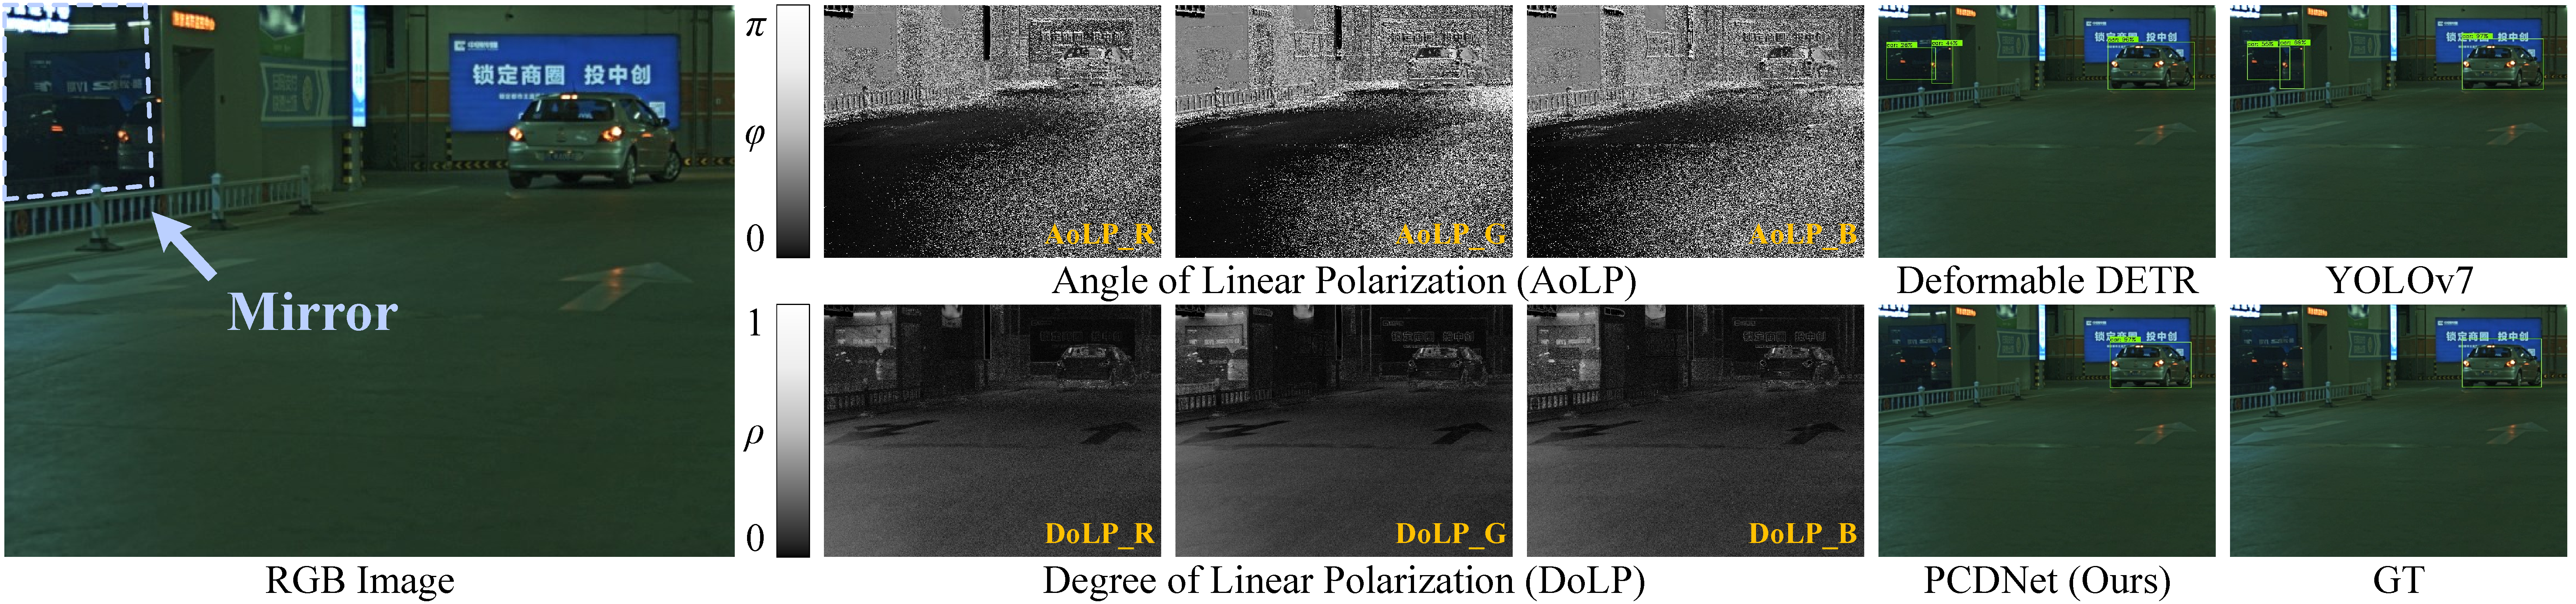
\includegraphics[width=\textwidth]{figure/teaser.pdf}
  \caption{Car detections (indicated by \dw{green} bounding boxes) obtained with the \textit{RGB-only} methods of Deformable DETR \cite{zhu2020deformable} and YOLOv7 \cite{wang2022yolov7} compared to our \textit{RGB-Polarization} Car Detection Network (PCDNet). Both prior methods fail to distinguish mirrored cars from real ones due to the similar visual appearances. In contrast, our method can handle such ambiguity and correctly detect the real car in scenes with the help of intrinsic material properties revealed by the polarization cues.}
  \label{fig:teaser}
\end{figure*}

\begin{abstract}
Car detection is an important task that serves as a crucial prerequisite for many automated driving functions. The large variations in lighting/weather conditions and vehicle densities of the scenes pose significant challenges to existing car detection algorithms to meet the highly accurate perception demand for safety, due to the unstable/limited color information, which impedes the extraction of meaningful/discriminative features of cars. In this work, we present a novel learning-based car detection method that leverages trichromatic linear polarization as an additional cue to disambiguate such challenging cases. A key observation is that polarization, characteristic of the light wave, can robustly describe intrinsic physical properties of the scene objects in various imaging conditions and is strongly linked to the nature of materials for cars (\textit{e.g.}, metal and glass) and their surrounding environment (\textit{e.g.}, soil and trees), thereby providing \textbf{\textit{reliable}} and \textbf{\textit{discriminative}} features for robust car detection in challenging scenes. To exploit polarization cues, we first construct a pixel-aligned RGB-Polarization car detection dataset, which we subsequently employ to train a novel multimodal fusion network. Our car detection network dynamically integrates RGB and polarization features in a request-and-complement manner and can explore the intrinsic material properties of cars across all learning samples. We extensively validate our method and demonstrate that it outperforms state-of-the-art detection methods. Experimental results show that polarization is a powerful cue for car detection. Our code is available at \url{https://github.com/wind1117/AAAI24-PCDNet}.
\end{abstract}

\section{Introduction}
Justice et al. \cite{justiceguide} state in their book that ``Children develop their knowledge of the world around them as they interact with their environment directly and indirectly. The direct experiences children have in their homes, schools and communities certainly provide the greatest amount of input to the world knowledge base.''. This knowledge arises from both physical and conversational interactions. In this paper, we test the hypothesis that just like a human child, machines need interaction to acquire world knowledge and develop commonsense reasoning abilities, and we study the effect of conversational interactions on this knowledge acquisition. Most of the literature on commonsense reasoning 
relies %rely [kmm- most-> relies]
on extracting the largest possible snapshot of 
%the [kmm- removed]
world knowledge and either 
query %query [kmm- on-> extracting and querying]
it or 
propose %propose [kmm- most-> proposes][could also parse as 'relies on-> proposing' or 'querying or proposing', may be better to restructure the sentence][fa- it was the later, so i restructured]
automated knowledge base completion methods for it. We argue that it is necessary to equip reasoning engines with an interaction strategy facilitating the extraction of just-in-time information needed for reasoning. 
%, through conversation with a human user [kmm- removed; conversation is covered by 'interaction' earlier in the sentence]
In this paper, we 
take up %take a few steps towards [kmm- rephrase (take steps/take steps repetitive)]
this grand goal, %[kmm- comma added]
and although we do not solve the whole challenge, we take the first steps needed for addressing it. 
Specifically, here we propose a ``soft'' commonsense reasoning engine and solve targeted knowledge base completion problems based on the information provided by the user through a conversational interface.

% We state this as our overarching grand research goal and mention carefully that we are taking a few steps towards this grand goal. Although it does not solve all of it but it is a step towards achieving this goal. This is just a first step however its a part of a very well reasoned and ambitious project. Then we also carefully describe the limitations of the project
% In other words, our overarching goal is having a human construct a reasoning system that does not have commonsense and extract commonsense from the user through conversation.
% \amoscomment{I think that it might be better saying something like: this work takes the first step towards ... I think that the paper could also benefit from adding a few sentences at the beginning.} \facomment{Is this resolved now?}

We believe that this is the right time for this proposal specifically since conversational agents such as Siri, Google home, Alexa and Cortana among others are starting to enter our daily lives. Therefore, it is plausible to assume that 
such agents %we [kmm- rephrase]
have access to conversation with a human for extracting commonsense knowledge. In this paper, we work with the Learning by Instruction Agent (LIA) \citep{azaria2016instructable,labutov2018lia} and develop a commonsense reasoning system for her called CORGI (\textbf{CO}mmonsense \textbf{R}easonin\textbf{G} by \textbf{I}nstruction). In what follows, we present our definition of commonsense reasoning for LIA after briefly introducing her. % It is worth noting, however, that the proposed method is not limited to a specific conversational agent. 
% \kmcomment{Anthropomorphizing LIA (referring to the agent as 'her') is a somewhat political choice -- it's okay to make it, but make it consciously.}

LIA is an intelligent agent that operates on 
a user's smartphone. %the phone [kmm- rephrase (you do not call LIA; there are other agents where you call in so it's important to make the distinction)]
%and can be taught new commands through user instructions. [kmm- removed (covered in the very next sentence)]
End users add new functionalities to LIA through verbal instructions and teach her how to perform new tasks. For example, the user can tell LIA, ``whenever it snows at night, wake me up 30 minutes early''. If LIA does not understand how to perform this task, she will ask the user to instruct her by breaking the task down into a set of steps in a teaching session. In this case, the user can say, ``(first) open the weather app, (second) see if the night weather condition is snow, (third) if true then adjust my alarm to 30 minutes earlier''. After this teaching session, LIA can perform this task. 

One phenomenon we have noticed in collecting these types of ``Whenever $S$ occurs, then do $A$'' instructions is that people often {\em underspecify} the precondition $S$. For example, one instructor might want to wake up early when it snows because they are concerned about getting to work on time.  For this user, the implied precondition is not really ``whenever it snows,'' but instead ``whenever it snows enough to cause traffic slowdowns, and it's a workday.'' The point is %Amos: I think that "the point is" doesn't sound good. How about "Naturally,"?
that people often fail to specify  such detailed conditions, perhaps because they are used to speaking to other people who possess the common sense needed to infer the more specific intent of the speaker.

Our goal for LIA is to use background commonsense knowledge to reason about the user's more specific intent, and to discuss this with the user in order to create the correct preconditions for the recommended action.  Therefore, we assume LIA can obtain statements from the user that fit the logical template ``Whenever $S$ occurs, do $A$ because I want to achieve goal $G$.''\footnote{Note in LIA's conversational setting, if the user gives an instruction of the form ``Whenever $S$ occurs, do $A$.'' and omits the reason, then LIA can simply respond ``Why do you want to do that?'' in order to prompt for the missing reason $G$.}
%LIA then generalizes from this statement to other actions. For example, if the user says, ``if the weather is rainy tomorrow then set an alarm for 1 hour later'', LIA can perform this action without needing to be taught again. However, this generalization has some limitations which 
%stem %stems [kmm- limitations->stem]
%from the lack of reasoning capabilities in LIA. 
For example consider the following two statements: %, [kmm- colon replaces comma]
\begin{itemize}
\item Whenever it snows at night, wake me up 30 minutes early because I don't want to be late to work
\item Whenever it snows at night, wake me up 30 minutes early because I have never seen the snow before 
\end{itemize}
Note that in the first statement, the user will not want to wake up early on a weekend or a holiday (assuming that they do not work then) whereas in the second scenario, the user will want to wake up early regardless of the date in order to see snow for the first time -- but might not want to wake up early once she has seen snow for the first time.

In CORGI, the role of commonsense reasoning is to derive the intended condition to use in place of the stated $S$ given an ``If $S$ then do $A$ because $G$'' statement from the user. Its general approach is to derive an explanation of how action $A$, performed in state $S$ will achieve goal $G$, and then to derive the intended precondition $S$ by collecting the preconditions on $S$ that allow this explanation to hold.  CORGI has access to a limited amount of general background knowledge about the world, represented in a logic programming language. Reasoning reduces to using this background knowledge to perform multi-hop logical inference. If no reasoning path is found, CORGI initiates a conversation with the user to extract relevant background knowledge and adds it to its underlying understanding of the world.  This newly acquired background knowledge will be used in future user interactions with CORGI. In essence, we are performing knowledge base completion through conversation, on a need-driven basis. Note that in earlier work Hixon et al. \cite{hixon2015learning} perform relation extraction using human interaction for question answering. Although the general idea of using human interaction is similar to our proposal, the information extraction method and the problem studied in \cite{hixon2015learning} differs from our setting. To the best of our knowledge, CORGI is the first conversational assistant that targets completing reasoning paths.
% \amoscomment{'their' seems like a typo, not sure what you are saying} --> resolved
% Therefore, our reasoning system is a commonsense reasoning by instruction engine. 

% \amoscomment{I find it hard to understand when 'LIA' refers to the agent from previous work, and when it refers to new capabilities added by this work.} \facomment{is this resolved now, Amos?} %Yes, Thanks!

% In this paper we develop a reasoning system for LIA that is capable of commonsense reasoning in order to generalize correctly given if-then user commands through the because statement.

CORGI's main reasoning component is the multi-hop inference system. Since the knowledge is represented in a logic programming language, the underlying inference algorithm is backward chaining. However, backward chaining in its traditional form is not robust to variations in natural language. This is specifically of importance since CORGI allows open-domain dialog with the user
to reduce the startup cost of the user having to learn a %so that the user is not limited to a [kmm- is this rephrase correct?]
specific grammar or vocabulary. Therefore, there is no parsing algorithm to resolve these variations. For example, in 
%the [kmm- removed]
traditional backward chaining, the statements ``if the forecast is snow tonight'' and ``if the weather is snowy tonight'' are thought of as two different statements whereas we want them both to map to the same representation. In order to address this, we propose a ``soft backward chaining'' algorithm that learns continuous representations or embeddings of the logical statements in the background knowledge. This will allow CORGI to indicate the equivalence of semantically similar statements based on the distance of their learned representations in the vector space. This soft backward chaining allows us to bridge a gap between symbolic AI and neural approaches using the best of both worlds.

% CORGI's soft backward chaining algorithm is end-to-end differentiable and is trained by looking at the proof traces of similar 

% kmm: resolve AA's confusion here with "compatible with deep-learning techniques"

% . This multi-hop reasoning system is end-to-end differentiable and supports soft multi-hop reasoning to account for natural language variations. \amoscomment{I might be missing something, but what does it mean being end-to-end differentiable, are you referring to differentiable functions (those that have a derivative), is this required in order to train the system? Or do you mean that the system obtains knowledge piece by piece. I guess you mean the former, but I did struggle with this.}

% \tmcomment{There are two main themes: 1. claiming that the reasoning can help get the generalization right, 2. how to do the reasoning in a way that is correct}

% \tmcomment{why are we doing reasoning this way and how can we make sure we can do it successfully. we need to compare it with the approximate inference and probabilistic inference methods for performing reasoning}

% \tmcomment{Our contributions are two fold. one is that we are proposing a reasoning strategy through conversation and are proposing to extract the missing information just in time to perform the correct reasoning. No one has the capacity to store the world's largest kb and until now everyone has tries to maintain the largest knowledge bases that there are. However, we are proposing a new way of doing this and it is to extract the correct part of the missing knowledge from the user. This is our grand goal and we have performed a set of small steps towards it... [layout the steps]. Another contribution is the soft unification part. In order to make this work we need to combine symbolic AI with neural approaches to bridge the gap and use the best of both worlds.}

% \tmcomment{reviewer question: How do we know if our method scales? No one has a large enough knowledge base that contains all the information there is in the world. And currently everyone in the field is trying to do this. However, we are proposing a method for extracting the right information just in time needed to perform the reasoning}

% \tmcomment{We do not know the user will give us the right answer even if we ask the right question} \kmcomment{Focus less on ``right'' answer/question here; there are many-to-many possible question/answer pairs that will give a good result. Make a definition of what success means in this context.}

% \tmcomment{Our goal is to have a conversation with the user and the main goal is to have the user give us the missing part of the information and in a funny/not so funny way this is a feature of the system}

% \tmcomment{consider the problem of learning procedures including triggers by conversation. When humans give instructions they are imprecise. In this project we are interested in having the human construct a reasoning system that does not have the commonsense and we want to use conversation to extract the commonsense from the user. We state this as our overarching grand research goal and mention carefully that we are taking a few steps towards this grand goal. Although it does not solve all of it but it is a step towards achieving this goal. This is just a first step however its a part of a very well reasoned and ambitious project. Then we also carefully describe the limitations of the project.}

\section{Background and Related Work}
\label{sec:related_work}

\textbf{Polarization} has a long research history in computer vision and is widely used in many tasks such as reflection removal \cite{wieschollek2018separating, lei2020polarized, li2020reflection}, surface normal and/or shape estimation \cite{chen2017multi, kadambi2015polarized}, and semantic segmentation \cite{mei2022glass, kalra2020deep}. Light is an electromagnetic wave, with its electric field oscillating perpendicularly to the direction of propagation. Unpolarized light has a randomly fluctuating electric field while polarized light has a biased direction of the electric field. Common light sources like the sun and LED spotlights emit unpolarized light which would become partially/fully polarized light when passing through a linear polarizer, reflecting off certain materials, or undergoing certain types of scattering.

In this work, we focus on the linear polarization measurement captured by the off-the-shelf polarization-array CMOS sensor which can record light intensities in four polarization directions, \textit{i.e.}, $I_{0^{\circ}}$, $I_{45^{\circ}}$, $I_{90^{\circ}}$, and $I_{135^{\circ}}$, respectively. The polarization state of the light can be described using the Stokes vector $S=[S_0, S_1, S_2, S_3]$, where $S_0$ stands for the total light intensity, $S_1$ and $S_2$ describe the ratio of the $0^{\circ}/45^{\circ}$ linear polarization over its perpendicular counterpart, and $S_3$ is the circular polarization power. The Stokes elements $S_0, S_1, S_2$ are formally defined as:
\begin{align} 
\label{eq:stokes}
\begin{array}{lr}
    S_0 =I_{0^{\circ}} + I_{90^{\circ}} = I_{45^{\circ}} + I_{135^{\circ}},\\
    S_1 =I_{0^{\circ}}-I_{90^{\circ}},\\
    S_2 =I_{45^{\circ}}-I_{135^{\circ}}.
\end{array}
\end{align}

The angle of linear polarization (AoLP) $\phi$ and the degree of linear polarization (DoLP) $\rho$ are then be calculated via:
\begin{align} 
\label{eq:polar}
    \phi = \frac{1}{2}arctan(\frac{S_2}{S_1}), \quad \rho = \frac{\sqrt{S_1^2+S_2^2}}{S_0}.
\end{align}

As shown in Fig. \ref{fig:samples}, the trees, walls or sky in the background usually exhibit a low linear polarization degree while the glass, rubber and plastic parts of a car are typically with a high linear polarization degree. This observation inspires us to exploit the material cues revealed by polarization for robust car detection.

\begin{figure*}[ht]
    \centering
    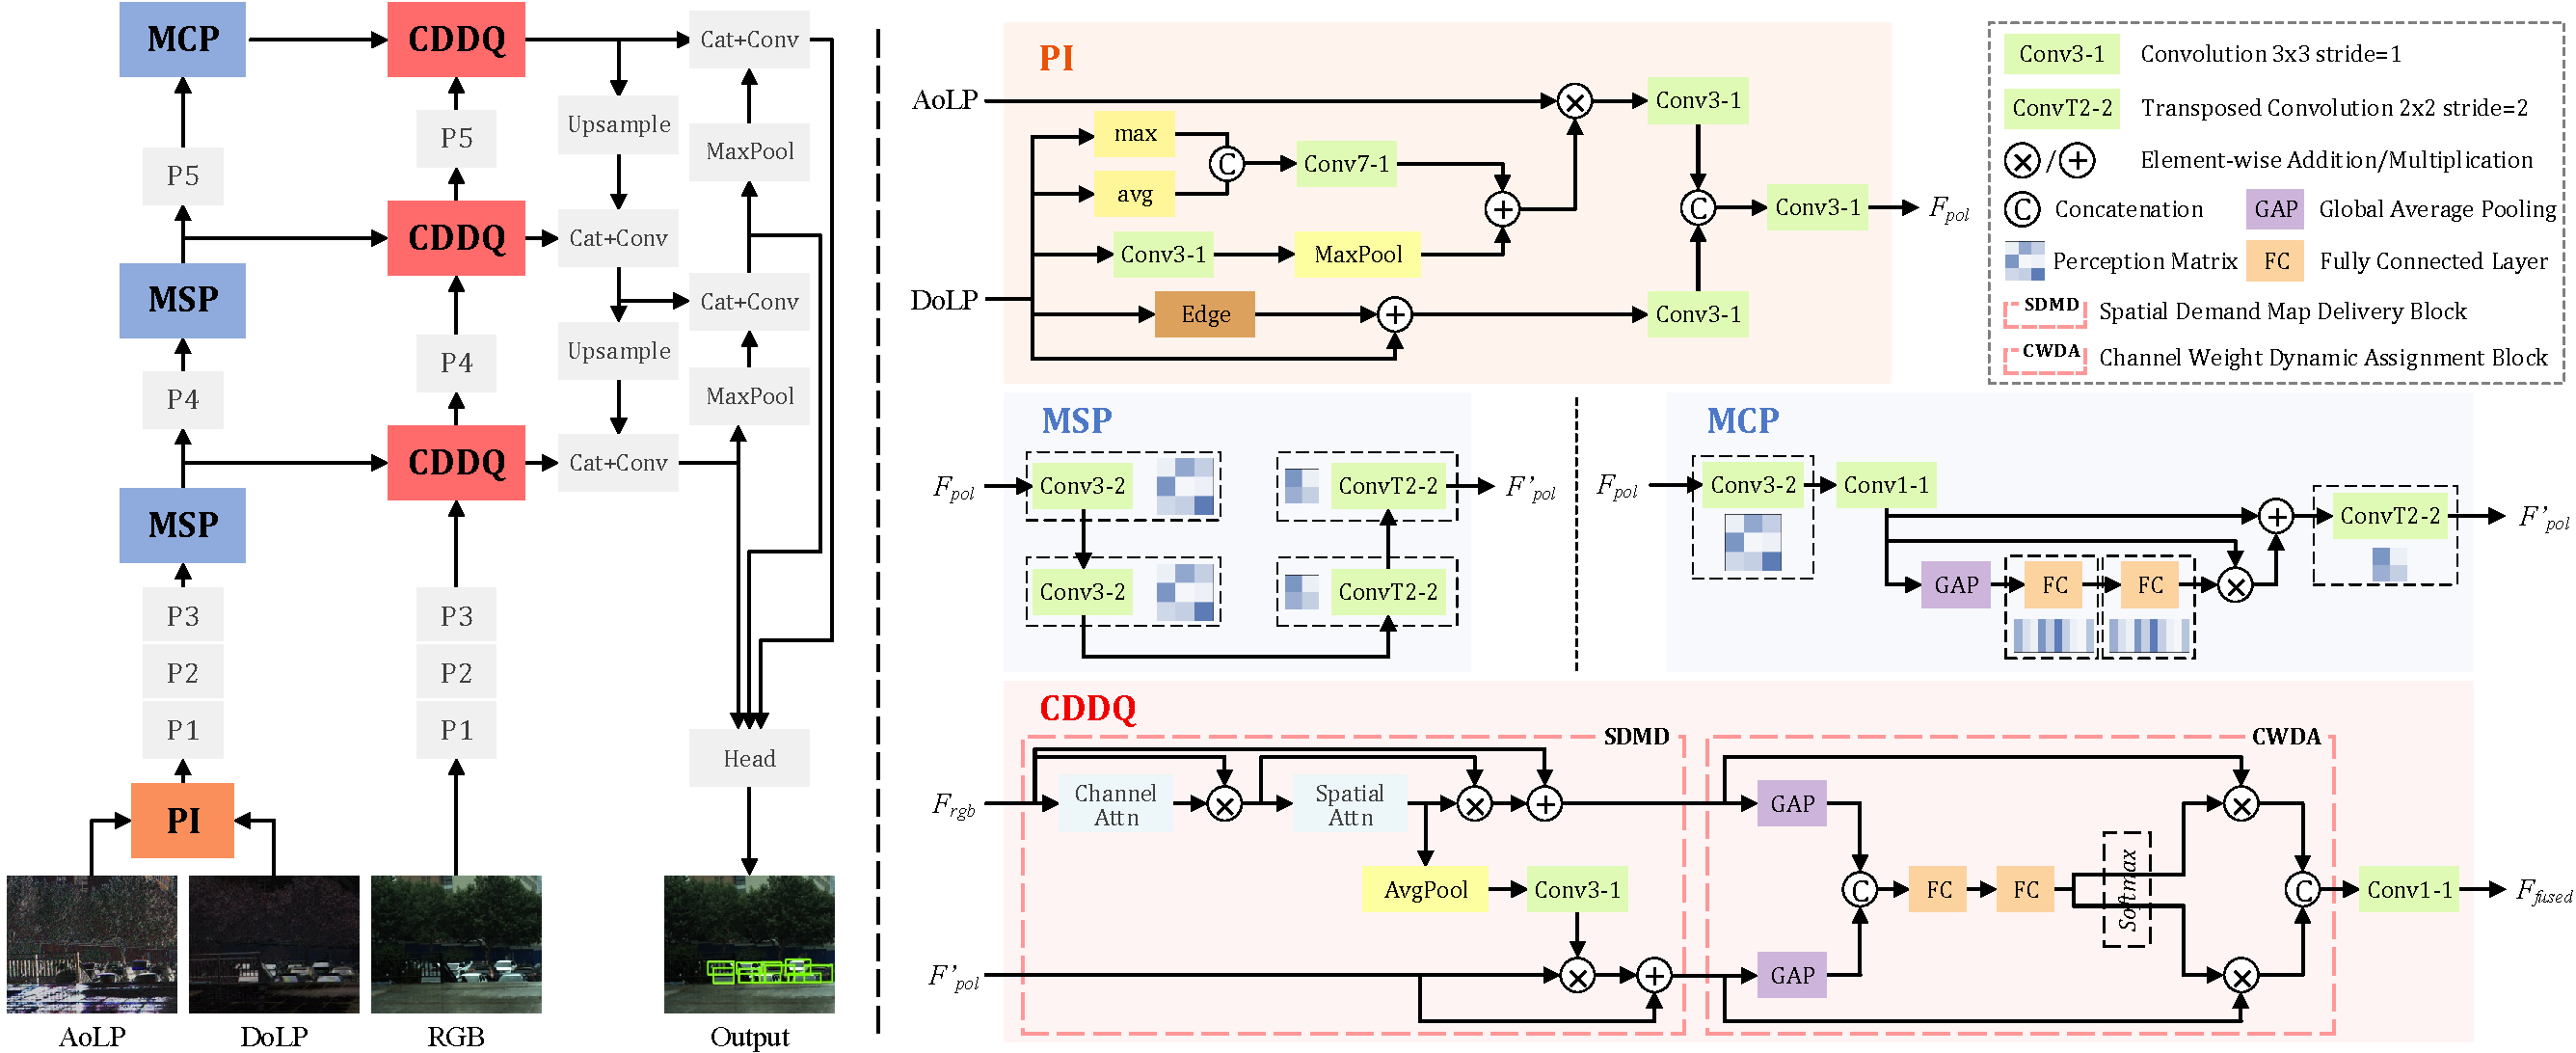
\includegraphics[width=\linewidth]{figure/methodology.pdf}
    \caption{Overview of PCDNet and its three main modules: the Polarization Integration (PI) module, the Material Spatial/Channel Perception (MSP/MCP) module, and the Cross Domain Demand Query (CDDQ) module.}
    \label{fig:pipeline}
\end{figure*}

\textbf{Object Detection} has achieved significant progress with the revolution of deep learning. Many state-of-the-art approaches emerged, including region-based detectors (\textit{e.g.}, Faster R-CNN \cite{Ren_2017} and EfficientDet \cite{tan2020efficientdet}), one-stage detectors (\textit{e.g.}, YOLO \cite{redmon2016you}, SSD \cite{liu2016ssd}, and RetinaNet \cite{lin2017focal}), and anchor-free detectors (\textit{e.g.}, FCOS \cite{tian2019fcos}). These methods typically employ advanced network architectures such as ResNet \cite{he2016deep}, VGG \cite{simonyan2014very} and EfficientNet \cite{tan2019efficientnet}. The trend in object detection has been toward the development of large models. The Vision Transformer \cite{dosovitskiy2020image}, derived from natural language processing \cite{zaheer2020big}, has achieved notable improvements in the field of object detection. For example, some methods such as Swin Transformer \cite{liu2021swin}, DETR \cite{carion2020end}, and DAB-DETR \cite{liu2022dabdetr} have achieved remarkable results on benchmark datasets including Microsoft COCO \cite{lin2014microsoft} and PASCAL VOC \cite{everingham2010pascal}. However, such models often exceed the hardware load and detection speed requirements of most restricted terminal devices. Moreover, most of them rely on clear and optimal RGB images which is hard to obtain in challenging scenes. Image enhancement and restoration on the low-quality RGB image will cost extra computing power and time. Our method differs from the above works in that we introduce reliable polarized material cues to complement traditional RGB features and design an RGB-P-based multimodal fusion network for robust detection.

\textbf{Multimodal Fusion} can provide rich contextual information for robust object detection \cite{valverde2021there, bijelic2020seeing}. Blin et al. employed a simple fusion method by stacking the multimodal data in the channel dimension to replace the original input \cite{blin2019road}. Manjunath et al. and Chen et al. adopted the concatenation \cite{manjunath2018radar} and element-wise addition \cite{chen2017multi} to fusing the low-level features of LiDAR and RGB, respectively. The attention mechanism \cite{vaswani2017attention} is also used to achieve multimodal fusion. HAFNet \cite{zhang2020hybrid} developed a cross-modal attention mechanism to perform feature fusion. Mei et al. calculated dynamic fusion weights for RGB and depth, considering the quality of each modality \cite{mei2021depth}. Similarly, Ji et al. used global average pooling followed by a fully connected layer to compute the channel attention weight for each modality \cite{ji2021calibrated}. Mei et al. generated spatial attention maps based on both global and local features to guide the multimodal fusion \cite{mei2022glass}. Although these methods achieve performance improvement to some extent, they perform information compensation in a passive ``post'' manner, resulting in the limited robustness of the model in challenging scenes. In this work, we develop a novel polarization material perception scheme to learn the intrinsic material properties of cars and a proactive multimodal fusion strategy to compensate RGB features with informative polarization cues in a ``request-and-complement'' manner, enhancing the robustness of car detection.


\section{Methodology}
\label{sec:methodology}
RGB images depict objects based on color differences that match human perception. However, objects with similar colors may not have enough color contrast to show their shape. By contrast, polarized light is strongly linked to the material of objects and the orientation of the reflecting surface, enabling it to reveal material properties that make object boundaries visible even when colors are similar (\textit{e.g.}, Fig. \ref{fig:samples} (a) and (b)). In spite of that, polarization cues may be weak in certain lighting conditions or viewing angles (\textit{e.g.}, Fig. \ref{fig:samples} (c)). Including polarization measurements naively in existing car detection methods may not necessarily yield the expected performance improvement. How to effectively integrate RGB and polarization features is a key challenge to be addressed to achieve robust car detection.

We introduce a novel Polarization Car Detection Network (PCDNet) that is capable of exploring and integrating polarized material cues for robust car detection. As shown in Fig. \ref{fig:pipeline}, PCDNet takes as input the RGB intensity, trichromatic AoLP and DoLP, and outputs car detections. The AoLP and DoLP are first integrated into a comprehensive and semantically meaningful polarization feature representation by a Polarization Integration (PI) module for the ease of the following feature extraction and fusion. Then, the RGB and polarization features are separately fed into two branches of CSPDarkNet \cite{wang2020cspnet} encoder, each consisting of five stages to extract multi-level contextual features. The Material Perception (MP) module, which aims to extract the intrinsic material properties of cars across the whole learning samples, is applied to different levels of extracted features. The MP module has a specific design for low-level features (MSP with spatial specialization) and high-level features (MCP with channel specialization), respectively. For multimodal feature fusion, the Cross-Domain Demand Query (CDDQ) module assigns fusion weights adaptively and conducts dynamic fusion in a request-and-complement manner. Finally, based on the fused features, we adopt the anchor-based detection head from YOLOv7 \cite{wang2022yolov7} to generate final classifications and bounding boxes.

\subsection{Polarization Integration (PI)}
AoLP $\phi$ and DoLP $\rho$ reveal object/scene materials from two different aspects. Polarization Integration (PI) module is designed to combine them into an unified and semantically meaningful polarization representation $F_{pol}$ for the ease of the following feature extraction and fusion. As the captured polarization angle is more likely random at regions with a low polarization degree, PI filters the AoLP measurement based on the DoLP. In addition, PI also extracts and integrates the edge information in DoLP measurement to help the distinction of objects with different materials. Formally,
\begin{align} \label{eq:pim}
    F_{pol} &=\vartheta_{3\cdot 1}([\vartheta_{3\cdot 1}(F_{\phi\rho}), \vartheta_{3\cdot 1}(\rho+\mathbb{E}(\rho))]), \\
    F_{\phi\rho} &=\phi\otimes(\vartheta_{3\cdot 1}([\hat{\mathbb{A}}(\rho),\hat{\mathbb{M}}(\rho)])+\sigma(\mathbb{M}(\vartheta_{3\cdot 1}(\rho)))),
\end{align}
where $\vartheta_{k\cdot s}$ denotes a $k \times k$ convolution with a stride of $s$, followed by a batch normalization and a SiLU activation function. $[\cdot]$ indicates the concatenation operation over the channel dimension. $\mathbb{E}$ refers to the Scharr edge extractor. $\otimes$ is the element-wise multiplication. $\hat{\mathbb{A}}$ and $\hat{\mathbb{M}}$ are the average and max pooling in the channel dimension, respectively. $\mathbb{M}$ is the max pooling in the spatial dimension with a kernel size of 5. And $\sigma$ is the Sigmoid activation.

\subsection{Material Perception (MP)}
Despite the cars in different scenarios may have diverse visual appearances such as different colors and textures, they are typically share similar materials including glass, rubber, metal, etc. Fortunately, polarization can robustly reveal the intrinsic physical properties of these materials. Inspired by this, we design the Material Perception (MP) strategy to explore
% and memorize 
the discriminative and invariant material features of cars across different scenarios. Considering the different characteristics of different levels of features, \textit{i.e.}, low-level features have larger spatial sizes and keep rich and detailed low-level information while high-level features contain more semantic cues distributed in more feature channels, MP is instantialized as Material Spatial/Channel Perception (MSP/MCP) modules for the low-/high-level polarization features, respectively. Formally, MSP/MCP can be described as:
\begin{align} \label{eq:mpm}
    MSP(F) &=\varrho_{2\cdot2}(\varrho_{2\cdot2}(\vartheta_{3\cdot2}(\vartheta_{3\cdot2}(F)))), \\
    MCP(F) &=\varrho_{2\cdot2}(\mathcal{M}((\vartheta_{1\cdot1}(\vartheta_{3\cdot2}(F))))), \\
    \mathcal{M}(x) &=x+x\otimes\sigma(m_2(m_1(\bar{\mathbb{A}}(x)))),
\end{align}
where $\varrho_{k\cdot s}$ denotes a $k \times k$ transposed convolution with a stride of $s$, followed by a batch normalization and a SiLU activation function. $\mathcal{M}(\cdot)$ is the perception scheme with two independent perception matrices in fully connected layers named $m_1$ and $m_2$. And $\bar{\mathbb{A}}$ is global average pooling.

\subsection{Cross Domain Demand Query (CDDQ)}
Polarization and RGB features are different types of representations of the scenes and simply combing them may dilute the useful clues of the cars originally presented in the individual modality or amplify the background interference. We address this issue by introducing the Cross-Domain Demand Query (CDDQ) module for effective multimodal feature fusion, taking into account both the context and quality of each modality feature. CDDQ takes as input the RGB features $F_{rgb}$ and polarization representations $F'_{pol}$. It first utilizes a Spatial Demand Map Delivery (SDMD) block to generate enhanced RGB features $F_{rgb}^{*}$ and distill informative and required polarization features $F_{pol}^{*}$ and then obtains fused features $F_{fused}$ through a Channel Weight Dynamic Assignment (CWDA) block:
\allowdisplaybreaks\begin{align}
    F_{rgb}^{*} &=F_{rgb}+F''_{rgb} = F_{rgb}+\mu\otimes F'_{rgb} \nonumber \\
        &=F_{rgb}+\mu\otimes \eta\otimes F_{rgb}, \\
    \eta &=\sigma(\vartheta_{1\cdot1}(\bar{\mathbb{M}}(F_{rgb}))+\vartheta_{1\cdot1}(\bar{\mathbb{A}}(F_{rgb}))), \\
% \end{align} 
% \begin{align}
    \mu &=\sigma(\vartheta_{7\cdot1}([\hat{\mathbb{A}}(F'_{rgb}), \hat{\mathbb{M}}(F'_{rgb})])), \\
    F_{pol}^{*} &=F'_{pol}+\vartheta_{3\cdot1}(\mathbb{A}(\mu))\otimes F'_{pol}, \\
    F_{fused} &=\vartheta_{1\cdot1}([\alpha\times F_{rgb}^{*},\beta\times F_{pol}^{*}]), \\
    \alpha, \beta &=\delta(\langle\sigma(fc(si(fc([\bar{\mathbb{A}}(F_{rgb}^{*}), \bar{\mathbb{A}}(F_{pol}^{*})]))))\rangle),
\end{align}
where $\eta$ is the channel attention vector. $\mu$ is the spatial attention map which also serves as the guidance of the informative polarization cues request process. $\mathbb{A}$ is an average pooling with a kernel size of 3. $\bar{\mathbb{M}}$/$\bar{\mathbb{A}}$ denotes global max/average pooling. $\alpha$ and $\beta$ are dynamic fusion weights assigned to the RGB and polarization features, respectively, with a constraint of being non-negative and summing up to 1 for each channel position. $fc$ is the fully connected layer and $\langle\cdot\rangle$ is the split operation over the channel dimension. $si$ and $\delta$ are the SiLU and Softmax activation functions, respectively.

\begin{figure}[ht]
    \begin{center}
        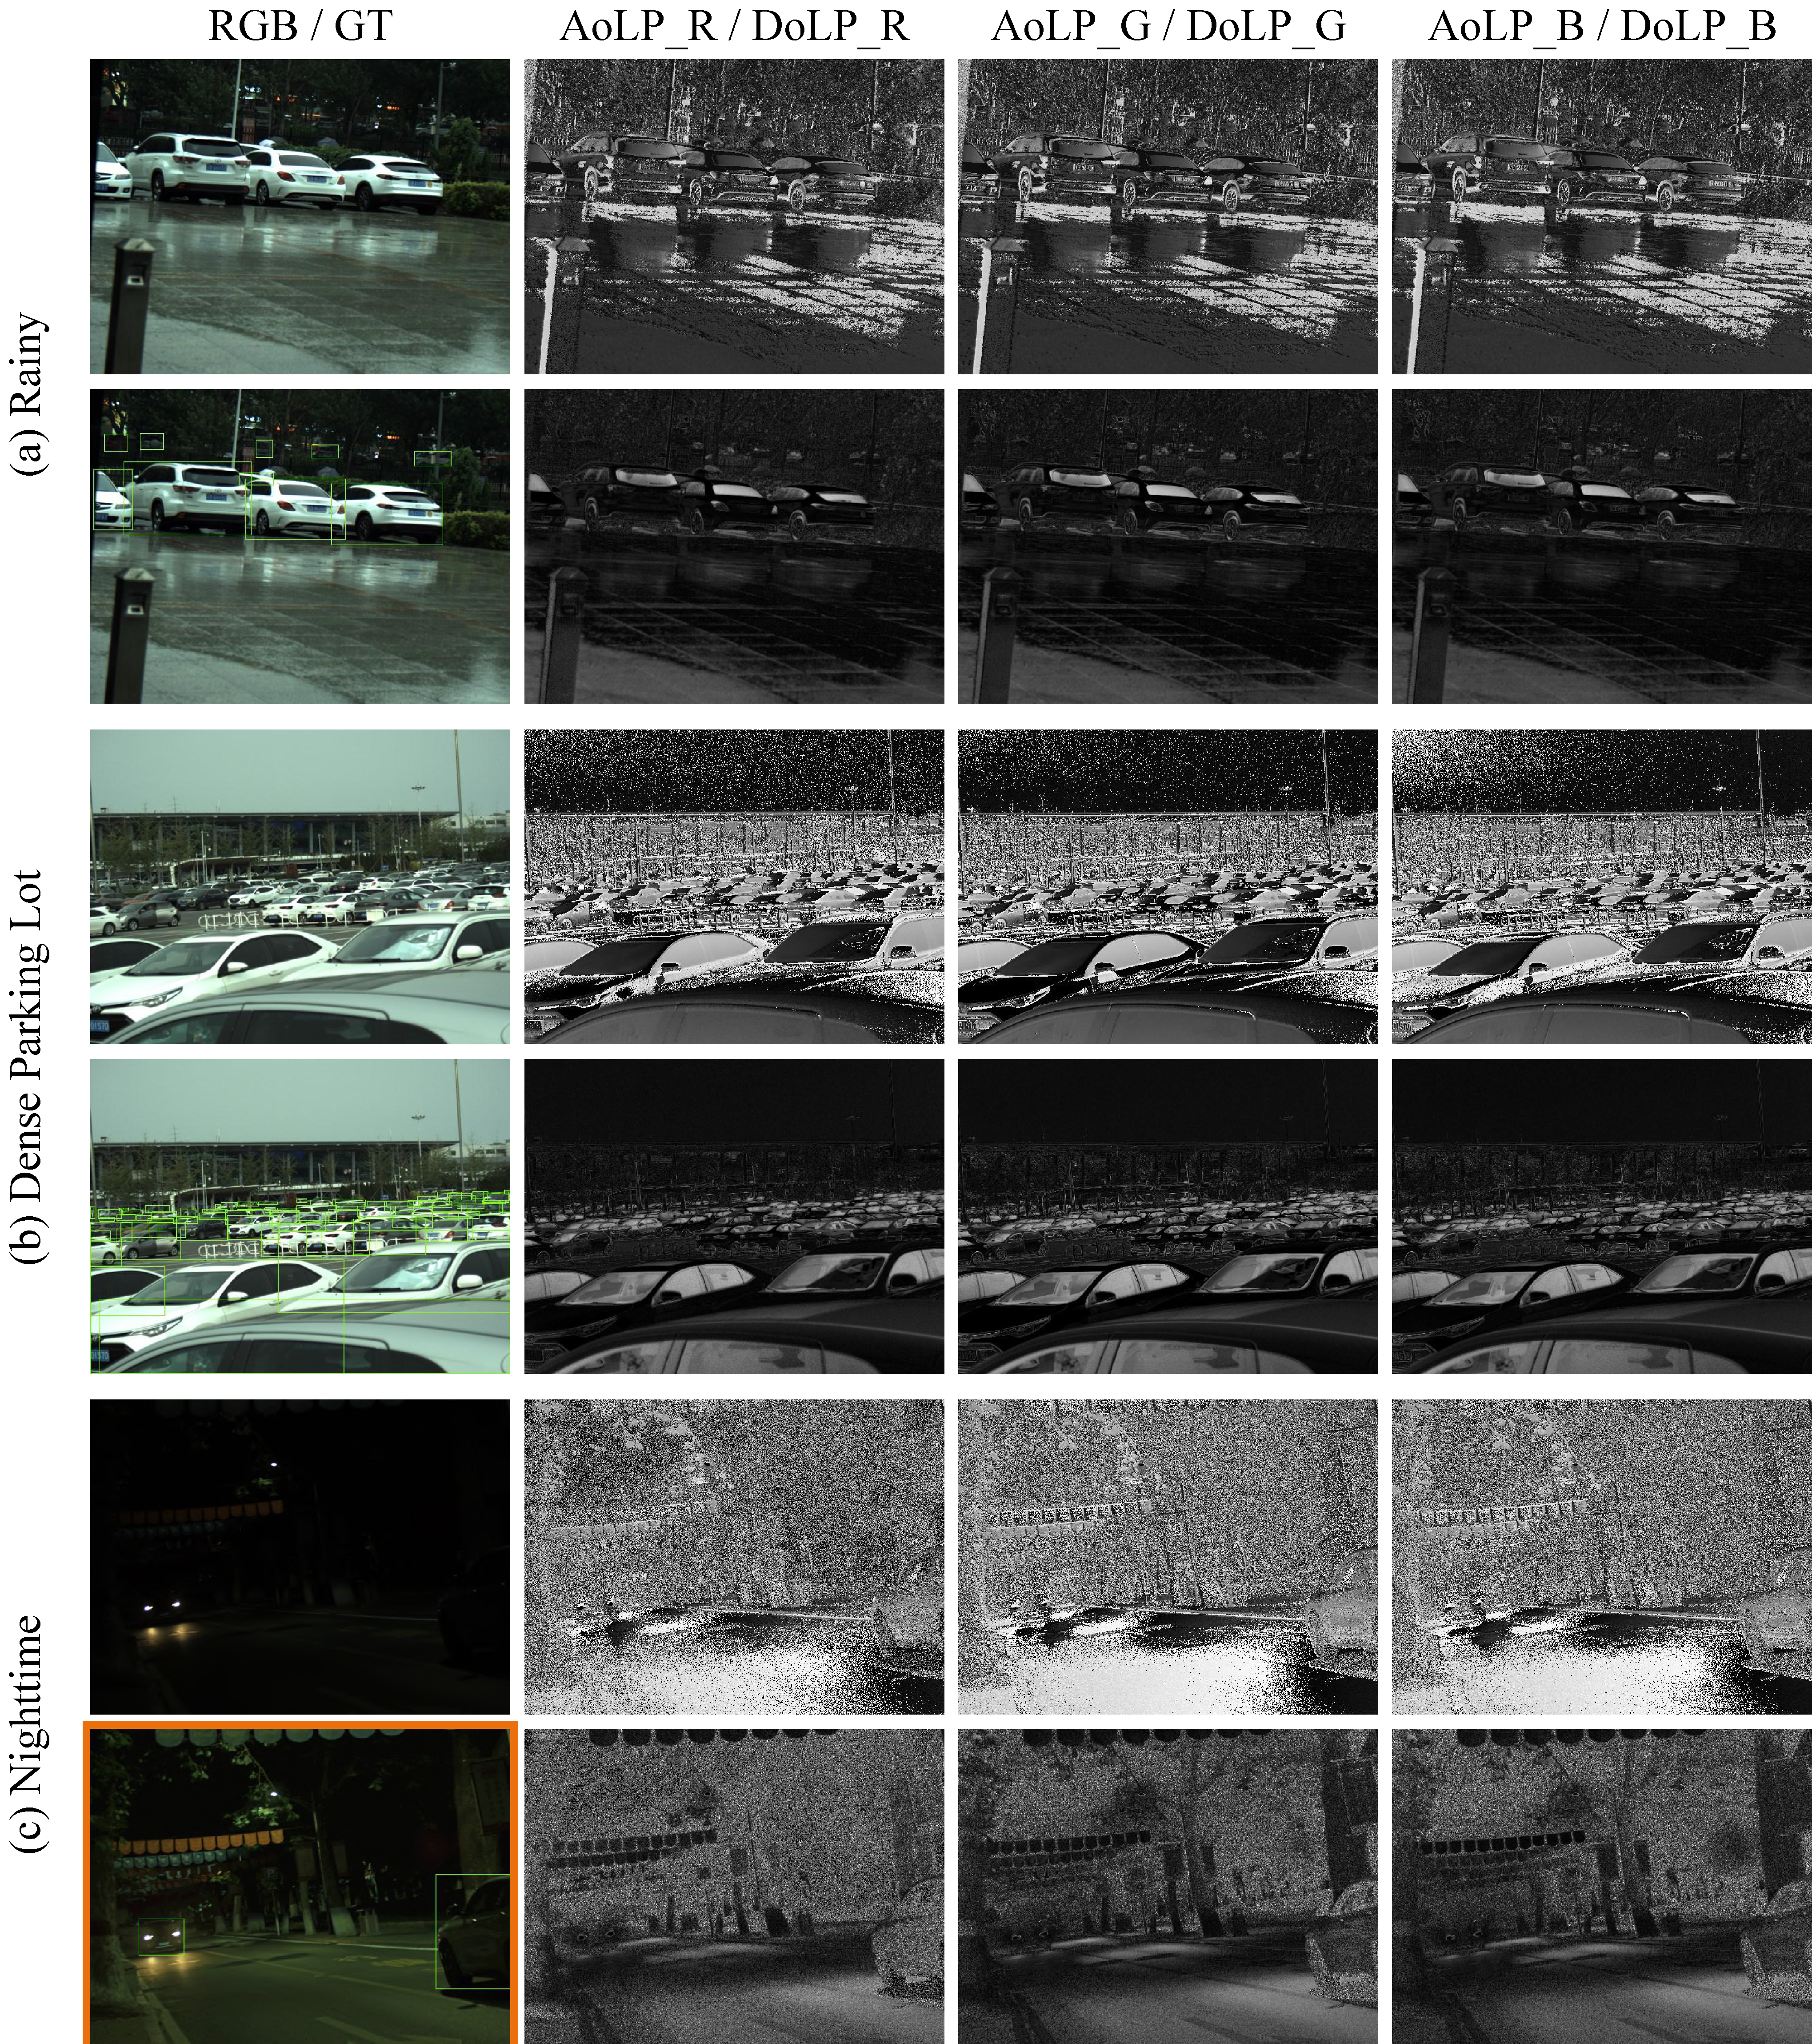
\includegraphics[width=1\linewidth]{figure/dataset.pdf}
    \end{center}
    \caption{
    RGBP-Car Examples. The first column displays the RGB intensity (top) and the corresponding annotation (bottom). The next three columns show the AoLP (top) and DoLP (bottom) measurements for the red, green, and blue channels, respectively. From top to bottom are scenes of stopped cars in a rainy parking lot, dense cars in an outdoor parking lot, and driving cars on a clear night road, respectively. 
    (The low-light RGB image is enhanced by ZeroDCE \cite{guo2020zero} (with \orange{orange} frame) for visualization.)}
    \label{fig:samples}
\end{figure}


\section{Task Formulation and Dataset}
\label{sec:datasets}
 
Fig. \ref{fig:neuronal-data} briefly illustrates the general pipeline of large-scale neuron reconstruction from EM image volume and various data used in our work.
The huge EM image volume is first over-segmented into a set of 3D segments using an off-the-shelf 3D segmentation approach. Subsequently, human proofreading is performed to obtain complete neurons that usually span several brain regions. The reconstructed neurons are commonly represented by tree structures composed of nodes and edges, either directly traced using annotation software such as CATMAID~\cite{saalfeld2009catmaid} or skeletonized from proofread segment surface using skeletonization algorithms such as TEASAR~\cite{sato2000teasar}. 
For each neuron, we register the over-segmented fragments with the neuron skeleton and obtain the connectivity relations between segments as the ground truth for training and testing.
 
In typical connectomics analysis workflows, human tracers start tracing from an interested neuron branch segment based on the over-segmentation results.
They identify the truncation point by examining its 3D surface mesh. Subsequently, they magnify the questionable area and determine which segment adjacent to the truncation point maintains neuronal continuity with the initial segment of interest, achieved by cross-referencing their 3D meshes and adjacent EM image slices.
For example, to trace the yellow branch in Fig.~\ref{dataset} (in the green box), a human tracer may zoom in to the terminal region, focusing on the lower-left image section. Then, the tracer transits to the adjacent section and sees that the area previously occupied by the yellow segment is now taken over by the blue segment, suggesting a potential connection between them. Typically, tracers proceed to verify their morphological continuity before merging.
   

To relieve the human proofreading workload for huge EM volumes, we propose to predict the connection probability of two segments, $S_a$ and $S_b$, considering their 3D morphology and the EM images from adjacent sections, mimicking the human tracing behavior. We learn the prediction function $f$ from a set of connected segment pairs ($f(S_a, S_b)=1$) that should be merged during proofreading and unconnected pairs ($f(S_a, S_b)=0$). 
 
\subsection{Dataset Construction}
 

\begin{table}[t]
    \caption{Overview of the datasets used in~\cite{matejek2019biologically} and our dataset \textbf{FlyTracing}. N/A denotes that the dataset is not public.
    }
    \centering
    \begin{tabular}{lS[table-format=1.1e2]lS[table-format=1.1e2]}
        \toprule
        \textbf{Dataset} & \textbf{Size ($\mu m^3$)} & \textbf{Method} & \textbf{\# Seg. Pairs} \\
        \midrule
        PNI & $\num{5.0e3}$ & Affinity & N/A \\
        Kasthuri & $\num{5.5e2}$ & Affinity & $\num{1.8e3}$ \\
        SNEMI3D & $\num{5.5e2}$ & Affinity & $\num{\sim e3}$ \\
        \textbf{FlyTracing} & $\num{3.2e6}$ & FFN & $\num{1.6e6}$ \\
        \bottomrule
    \end{tabular}
    \label{dataset-compare}
\end{table}

 \subsubsection{Dataset Overview.}
Available datasets for neural segment connection tasks mainly originated from densely annotated blocks, limited in scale and diversity. 
In contrast, we extract segment connectivity from the crowd-sourced proofreading results throughout an entire fly brain. 
As Table \ref{dataset-compare} shows, our dataset \textbf{FlyTracing} surpasses existing datasets by three orders of magnitude, regarding the volume size and number of connected segment pairs.
The source EM images for FlyTracing are from a complete adult Drosophila brain, imaged at $4\times4 nm$ resolution and sectioned with the thickness of $40 nm$, known as the “full adult fly brain” (FAFB) dataset~\cite{FAFB}. The image sections are first preprocessed through local re-alignment and irregular section substitution, and segmented through a multi-scale FFN segmentation pipeline~\cite{fafb-ffn}, referred to as FAFB-FFN1. The proofread neuron skeletons are supplied by FlyWire~\cite{dorkenwald2022flywire}. 
Despite the availability of affinity-based automatic segmentation from FlyWire, we choose FAFB-FFN1 due to its adherence to over-segmentation consensus, i.e., fewer merging errors than affinity-based segmentation results. 

 \subsubsection{Segment-Neuron Registration.} 
 To generate the ground truth of connectivities of EM segment pairs, we register the FFN segmentation results with the proofread neuron skeletons.
 We design an automatic EM segment-neuron registration method that can be applied to any large-scale connectomics datasets with proofread neuron skeletons and over-segmentation results. 
 With permission from Flywire, we obtain the surface meshes of the proofread neurons and skeletonize them using the skeletor tool~\cite{philipp_schlegel_2022_7308283}. 
 Since we focus on tracing neurites with tree-like structures, we cut off the cell body fibers from the neuron segments.

 
To register the massive over-segmented fragments with a human proofread neuron, given its neuron skeleton $T_{n}$, we associate each skeleton node with its nearest segment.
Since the extracted skeletons and EM image segmentation results inevitably contain errors and noises, a few nodes are occasionally assigned to segments that do not belong to the right neuron. 
To mitigate the assignment errors, we calculate the chamfer distance from the segment skeleton $T_{S}$ to the neuron skeleton $T_{neu}$, subsequently discarding the segments and their corresponding nodes whose $CD(T_{S}, T_{neu})>2\bar{r}$. 
Here, $\bar{r}$ denotes the estimated average radius of the local branch: $\bar{r} = \frac{1}{ |\Omega_S|} \sum_{i\in \Omega_S} r_i$, where $\Omega_S$ is the set of all the neuron skeleton nodes associated to segment $S$. 
%
Once every node is assigned with a corresponding segment, we traverse along the neuron skeleton and identify edges between nodes that are assigned to different segments as bridging edges:
\begin{equation}
    E_{bridge}(T_{neu}) = \{edge(\mathbf{v}_i, \mathbf{v}_j)| S_a \neq S_b\},
\end{equation}
where $\mathbf{v}_i$, $\mathbf{v}_j$ represent two adjacent nodes in $T_{neu}$, and $S_a,S_b$ are their corresponding segments, indicating $S_a$ and $S_b$ should be merged as the same neuron via $edge(\mathbf{v}_i,\mathbf{v}_j)$. 
%
\begin{figure}[t]
    \centering
    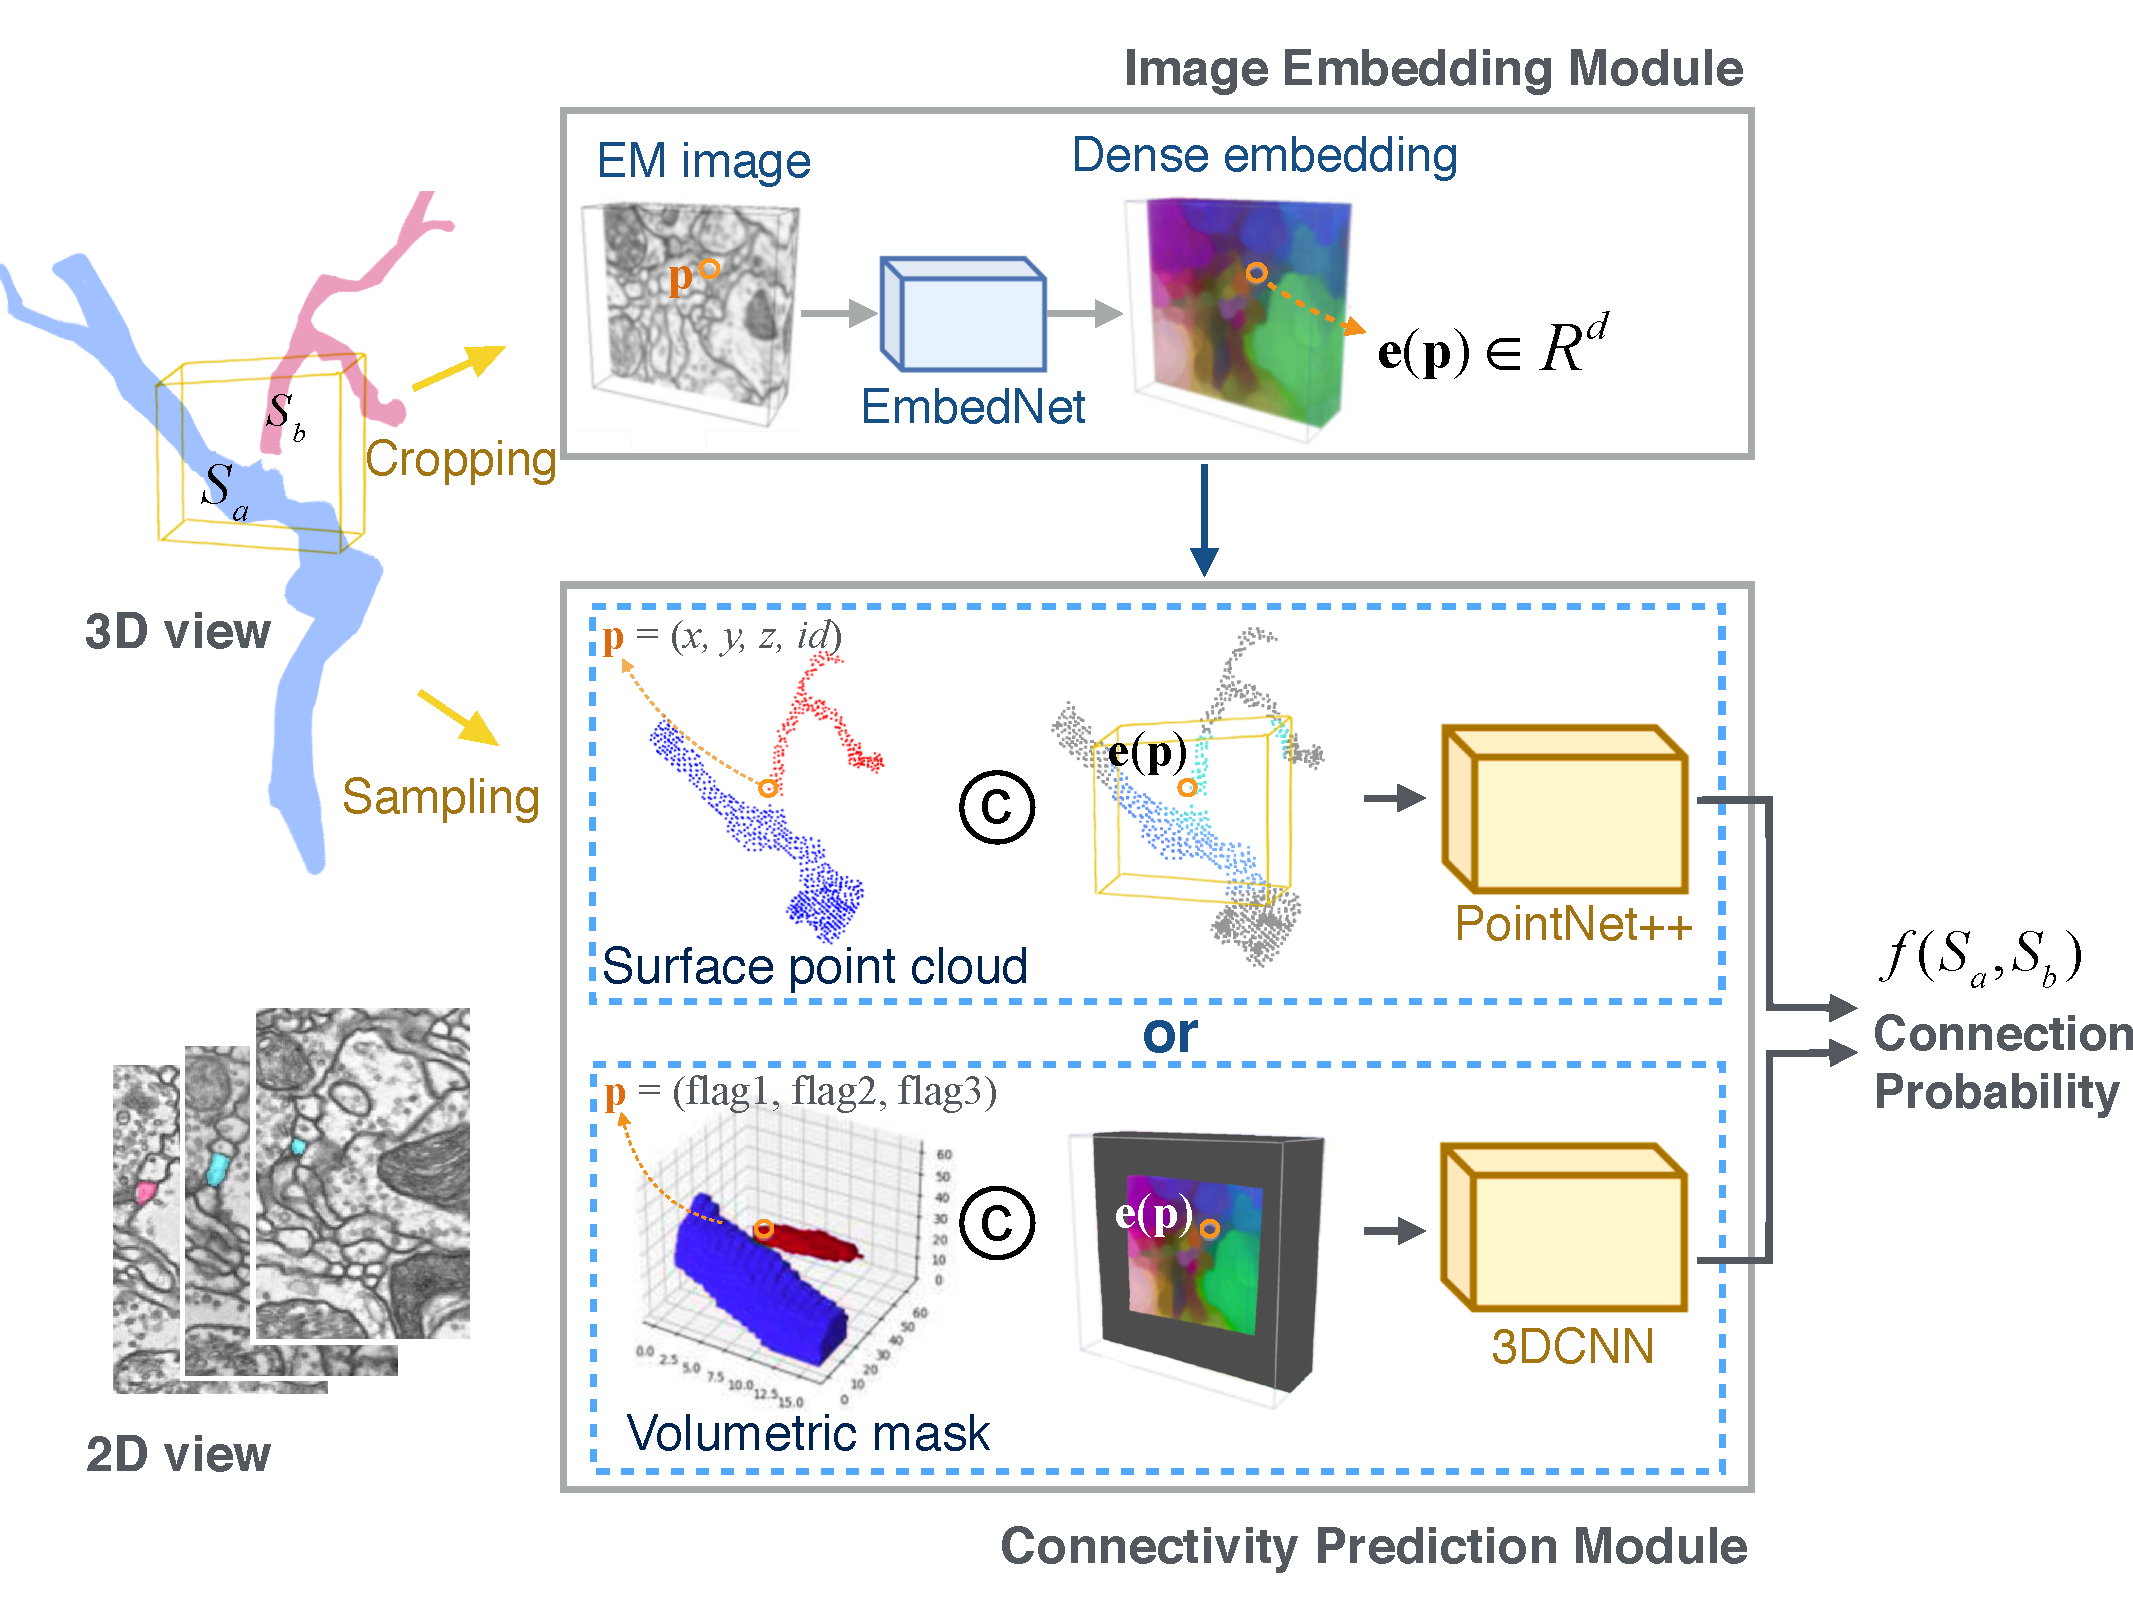
\includegraphics[width=0.48\textwidth]{figs/3Dmodel.pdf}
    \caption{Our connectivity prediction framework fuses local volumetric image features extracted by the EmbedNet with 3D morphology, optionally represented by point cloud or volumetric masks.}% 
    \label{fig:3Dmodel}
\end{figure}

Consequently, we collect the entire bridging edge set from $23,769$ proofread neurons.
The average count of bridging edges per neuron is 810. 
%
For each bridging edge $edge(\mathbf{v}_i, \mathbf{v}_j)$, assuming ${\mathbf{c}}_{i,j}$ is the midpoint of $\mathbf{v}_i$ and $\mathbf{v}_j$, we add random shift to the coordinate of ${\mathbf{c}}_{i,j}$ and obtain ${\hat{\mathbf{c}}}_{i,j}$ as the estimated truncated point. 
The segment pair $(S_a, S_b)$ is annotated as a positive connecting pair ($f(S_a, S_b)=1$).
Any segment $S_c$ that is located in the cube of size $H\times W\times D$ centered at ${\hat{\mathbf{c}}}_{i,j}$ and $S_c \neq S_b$ is labeled with $S_a$ as a negative pair ($f(S_a, S_c)=0$). 


 \subsubsection{Training and Test Block Partition.}
The positive segment pairs across the entire fly brain are partitioned into blocks based on their location in the brain, each spanning a volume size of $26\times 26\times 1\mu m^3$. We select $4,000$ blocks, each of which contains a minimum of $350$ positive segment pairs for training and testing. 
 $1,000$ blocks are selected randomly as the training and validation set for the image embedding network and pairwise connectivity prediction models. The rest $3,000$ blocks are used for testing of connectivity prediction.
 
 


\section{Experiments}
\label{sec:experiment}

\begin{table}[t]
\centering
\small
\resizebox{0.99\linewidth}{!}{
\begin{tabular}{lcccc}
\multirow{2}{1.5cm}{\textbf{Methods}} & \multicolumn{2}{c}{\textbf{Far-OOD}} & \multicolumn{2}{c}{\textbf{Near-OOD}}\\
\cmidrule{2-5}
& \textbf{FPR95}  & \textbf{AUROC} & \textbf{FPR95}  & \textbf{AUROC}\\
& $\downarrow$ & $\uparrow$ & $\downarrow$ & $\uparrow$ \\
\toprule
\emph{Using model outputs}\\
MSP~\cite{hendrycks2016baseline} & 52.11 & 91.79 & 64.66 & 85.28 \\
ODIN~\cite{liang2018enhancing}  & 26.47 & 94.48 & 52.32 & 88.90\\
GODIN~\cite{hsu2020generalized}  & 17.42  & 95.84 & 60.69 & 82.37 \\
Energy score~\cite{liu2020energy}  & 28.40 & 94.22 & 50.64 & 88.66 \\
ReAct~\cite{sun2021react} & 33.12 & 94.32 & 53.51 & 88.96\\
GradNorm~\cite{huang2021importance} & 24.79 & 92.58 & 65.44 & 79.31\\
LogitNorm~\cite{wei2022mitigating}  & 19.61 & 95.51 & 55.08 & 88.03\\
DICE~\cite{sun2022dice}  & 20.83 & 95.24 & 58.60 & 87.11 \\
\midrule
\emph{Using feature representations}\\
Mahalanobis~\cite{lee2018simple} & 44.55 & 82.56 & 87.71 & 78.93 \\
KNN~\cite{sun2022knn}  & 18.50 & 96.36 & 58.34 & 87.90 \\
\midrule 
 \name (ours) & \textbf{14.99} & \textbf{97.15}  & \textbf{50.10} &  \textbf{89.80}\\
 & $\pm{0.87}$ & $\pm{0.27}$ & $\pm{1.09}$ & $\pm{0.65}$\\
\bottomrule
\end{tabular}}
\caption{\small Performance comparison on near-OOD and far-OOD detection task. Architecture used is DenseNet-101 and ID data is CIFAR-10. We report the mean and variance across 3 training runs.}
\label{tab:hard_ood}
\end{table}
\begin{table}[t]
\small
\centering
\resizebox{0.99\linewidth}{!}{
\begin{tabular}{lccc}
\textbf{Method} & \textbf{FPR95}  & \textbf{AUROC} & \textbf{ID Acc.}\\
& $\downarrow$ & $\uparrow$ & $\uparrow$ \\
\toprule
\emph{Methods using model outputs}\\
MSP~\cite{hendrycks2016baseline} & 77.59 & 76.47 &  75.14\\
ODIN~\cite{liang2018enhancing} & 56.39 & 86.02 & 75.14\\
GODIN~\cite{hsu2020generalized} & 44.08 &  89.05 & 74.37\\
Energy score~\cite{liu2020energy} & 57.07 &  84.83 &  75.14\\
ReAct~\cite{sun2021react} & 75.06 & 79.51 & 66.56\\
GradNorm~\cite{huang2021importance} & 63.05 & 79.80 & 75.14\\
LogitNorm~\cite{wei2022mitigating} & 61.10 & 84.72 & 75.42\\
DICE~\cite{sun2022dice} & 49.72 & 87.23 & 68.65 \\
\midrule 
\emph{Methods using feature representations}\\
Mahalanobis~\cite{lee2018simple} & 56.93 & 80.27 &  75.14\\
KNN~\cite{sun2022knn} & 47.21 & 85.27 & 75.14\\
\midrule 
 \name (ours) & \textbf{31.25} & \textbf{90.76} & \textbf{75.59}\\
& $\pm{1.25}$ & $\pm{0.36}$ & $\pm{0.08}$\\
\bottomrule
\end{tabular}}
\caption{\small Performance comparison on CIFAR-100 dataset. We use DenseNet-101 for all baselines. Best  results are in \textbf{bold}. We report the mean and variance across 3 different training runs.}
\label{tab:cifar-100}
\end{table}
In this section, we extensively evaluate the effectiveness of our proposed method. 
The goal of our experimental sections is to mainly answer the following questions: (1) Can \name alleviate the curse of dimensionality? (2) How does \name compare against the state-of-the-art OOD detection methods?  Due to space constraints, extensive experimental details are in Appendix C. Our code is open-sourced for the research community.


\subsection{Evaluation on Common Benchmarks}
\label{subsec:common_benchmark}

\noindent \textbf{Datasets.} In this section, we make use of commonly studied CIFAR-10 (10 classes) and CIFAR-100 (100 classes)~\cite{krizhevsky2009learning} datasets as ID. Both datasets consist of images of size $32 \times 32$. We use the standard split with $50,000$ images for training and $10,000$ images for testing. We evaluate the methods on common OOD datasets: \texttt{Textures}~\cite{cimpoi2014describing}, \texttt{SVHN}~\cite{svhn}, \texttt{LSUN-Crop}~\cite{yu2015lsun}, \texttt{LSUN-Resize}~\cite{yu2015lsun}, \texttt{iSUN}~\cite{xu2015turkergaze}, and \texttt{Places365}~\cite{zhou2017places}. Images in all these test datasets are of size $32 \times 32$. 


\paragraph{Evaluation metrics.} We compare the performance of various methods using the following metrics: 
(1) {FPR95} measures the false positive rate (FPR) of OOD samples when $95\%$ of ID samples are correctly classified;
(2) {AUROC} is the area under the Receiver Operating Characteristic curve; 
and (3) {ID Acc.} measures the ID classification accuracy.

\vspace{0.2cm}
\noindent \textbf{Comparison with competitive methods.} In Table~\ref{tab:cifar-100}, we provide a comprehensive comparison with competitive OOD detection baselines on  CIFAR-100. {We provide a detailed description of baseline approaches in Appendix C.3.} We observe that our proposed method \name significantly outperforms the latest rivals. For a fair comparison, we divide the baselines into two categories: methods using model outputs and methods using feature representations.
From Table~\ref{tab:cifar-100}, we highlight two salient observations: (1) Considering methods based on feature representations, \name outperforms KNN (non-parametric) and Mahalanobis (parametric) by \textbf{15.96\%} and \textbf{25.68\%} respectively in terms on FPR95. The results validate that learning feature subspace effectively alleviates the ``curse-of-dimensionality" problem that is troubling the existing KNN approach. (2) Further, \name also performs better than output-based methods such as ReAct~\cite{sun2021react}. Specifically, with CIFAR-100 as ID, \name provides a $\mathbf{43.81}\%$ improvement in FPR95 as compared to ReAct~\cite{sun2021react}. Notably, \name provides a \textbf{18.47\%} improvement compared to~\cite{sun2022dice}, a post-hoc sparsification method. While DICE can severely affect the ID test accuracy (68.65\%), \name exhibits stronger classification performance (75.59\%) by baking in the inductive bias of subspaces through training. An extensive discussion is provided in Section~\ref{sec:discussion}. 



\paragraph{Evaluation on near-OOD data.} In Table~\ref{tab:hard_ood}, we compare the performance in detecting near-OOD data, which refers to samples near the ID data. Near-OOD is particularly challenging to detect, and can often be misclassified as ID. We report the performance on CIFAR-10 (ID) vs. CIFAR-100 (OOD), which is the most commonly used dataset pair for this task. We observe that \name consistently outperforms existing algorithms for near-OOD detection tasks, further demonstrating its strengths. Compared to KNN, \name reduces the FPR95 by 8.24\%. For completeness, we also provide far-OOD evaluation results on CIFAR-10, where \name achieves an average FPR95 of 14.99\%. Full result on each test dataset for CIFAR-10 is available in Appendix D.4.



\begin{table}[t]
\small
\centering
\resizebox{0.95\linewidth}{!}{
\begin{tabular}{lccc}
\textbf{Method} & \textbf{Dataset (ID)} & \textbf{FPR95}  & \textbf{AUROC} \\
& & $\downarrow$ & $\uparrow$  \\
\toprule
Mahalanobis~\cite{lee2018simple} & CIFAR-10 & 44.55 & 82.56  \\

\name (w. Mahalanobis) & CIFAR-10 &  \textbf{34.68} &  \textbf{87.87} \\
\midrule
Mahalanobis~\cite{lee2018simple} & CIFAR-100 & 56.93 & 80.27  \\

\name (w. Mahalanobis) & CIFAR-100 &  \textbf{55.05} &  \textbf{80.77} \\
\bottomrule
\end{tabular}}
\caption{\small \name is also compatible with parametric approaches such as Mahalanobis distance~\cite{lee2018simple}. The model is DenseNet. All values are averaged over six OOD test datasets.}
\label{tab:compatibility}
\end{table}


\paragraph{Compatibility with other distance-based approaches.} 

Beyond KNN~\cite{sun2022knn}, the Mahalanobis distances~\cite{lee2018simple} is also one of the most popular distance-based approaches to detect OOD. 
However, all prior solutions measure the distance with a full feature space which can also suffer from the curse of dimensionality. 
In this section, we show that subspace learning can also benefit parametric approaches like Mahalanobis distance~\cite{lee2018simple}. In Table~\ref{tab:compatibility}, we compare the OOD detection performance of using Mahalanobis distance on the vanilla model and the model trained with \name. 
We see that coupling subspace learning (in training) with Mahalanobis distance (in testing) reduces FPR95 by {9.87\%} and {1.88\%} on CIFAR-10 and CIFAR-100 datasets respectively.

\begin{table}[t]
\small
\centering
\resizebox{0.55\linewidth}{!}{
\begin{tabular}{lcc}
\toprule
\multirow{2}{2cm}{\textbf{Training Method}} &  CIFAR-10 & CIFAR-100 \\ 
& \multicolumn{2}{c}{(Train time in hours)} \\
\midrule
Standard & $2.10$ & $2.25$\\ 
 \name & $1.75$ & $1.89$ \\
\bottomrule
\end{tabular}}
\caption{\small \textbf{Computational cost for training}. trained using ResNet-101. 
Model used is DenseNet-101. For the comparison, we used the software configuration as reported in Appendix C.2.}
\label{tab:train_time}
\end{table}
% 
\paragraph{Computational complexity.}  In Table~\ref{tab:train_time}, we compare the training time of \name with the standard training method using cross-entropy loss. We observe that training using \name incurs no additional computation overhead but rather is slightly more efficient compared to standard training procedures. This is because we perform gradient descent only on a subset of weights corresponding to the selected feature subspace. Thus, our method overall leads to faster updates and convergence. {In Appendix D.1, we further show that
\name remains competitive and outperforms the KNN counterpart on other common architecture.}

\section{Conclusion}
In this paper, we introduced a new ad-hoc retrieval approach GRMM which explicitly incorporates document-level word relationships into the matching function. The flexible graph structure allows the model to find more comprehensive matching patterns and less noises. GRMM exceedingly advances the performance over various baselines, where it empirically witnesses an increment by a large margin on longer documents. Further studies exhibited the rationality and effectiveness of GRMM. There are also possible extensions, such as training with large click logs \cite{jiang2016learning} and query descriptions. Another interesting future work is to extend the current graph with lexical or knowledge graphs which might contain more useful information. 

\bibliography{aaai24}

\end{document}
